%\documentclass[12pt]{report} %,twoside
%\usepackage{kjfsty}
%
%\usepackage{multibib}
%\newcites{sec}{ }
%
%\begin{document}
%\tableofcontents
%
%\onehalfspacing
%
%
%%\renewcommand{\sfdefault}{phv}
%%\renewcommand{\rmdefault}{ptm}
%%\renewcommand{\ttdefault}{pcr}
%

\setcounter{chapter}{2}
\chapter[ZnCdSe/ZnCdMgSe Quantum Cascade Emitters]{ZnCdSe/ZnCdMgSe \\ Quantum Cascade Emitters}

\glossary{name={QC}, description={quantum cascade}, sort=q}
\glossary{name={QCL}, description={quantum cascade laser}, sort=q}
\glossary{name={CW}, description={continuous wave}, sort=c}
\glossary{name={RT}, description={room temperature}, sort=r}
\glossary{name={ICL}, description={interband cascade laser}, sort=i}
\glossary{name={DFB}, description={distributed feedback}}
\glossary{name={FTIR}, description={Fourier transform infrared spectrometer}}
\glossary{name={MBE}, description={molecular beam epitaxy}}
\glossary{name={LO}, description={longitudinal optical}}
\glossary{name={SEM}, description={scanning electron microscope}}

Among the present-day challenges for light emitters are ``gaps'' in the spectrum where high quality (room temperature and CW) laser sources are commercially unavailable.  Even when considering cutting-edge devices produced by research institutions, key gaps in coverage remain.  Of particular immediate interest is the break between the current capabilities of diode lasers and QC lasers---between about 3--4~\um.  This technological break inconveniently consumes a large part of the so-called first atmospheric window, the wavelength range from about 3--5~\um\ where there is minimal atmospheric absorption.  Illustrated in Fig.~\ref{chpt2:first_window}, this is also the domain of primary ro--vibrational absorption resonances for many important molecular species of academic and industrial interest, especially the C--H stretch.

\begin{figure}[tbp]
\centering
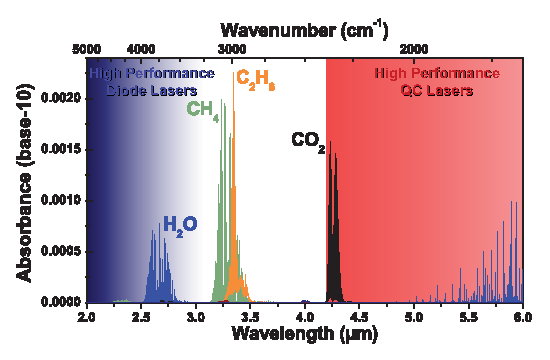
\includegraphics[width=5in]{chpt2/first_window}
\caption[Absorption spectra and laser capabilities near the first atmospheric window.]{\textnormal{\textbf{Absorption spectra and laser capabilities near the first atmospheric window.}}  Many important molecular species, such as methane and ethane, have ideally strong absorption resonances in the first atmospheric window.  Today's commercially available high-performance light sources are unable to cover many of these important wavelengths.}
\label{chpt2:first_window}
\end{figure}

The gap, however, is closing; three technologies are currently in competition to claim title to this space.  Using InGaAsSb wells and AlInGaAsSb quinternary barriers, quantum well diode lasers approaching from the short-wavelength side have reached $\lambda$~=~3.36~\um\ at 12~$^{\circ}$C with 15~mW of CW output power \cite{Shterengas:APL:2008}.  Because of the small semiconductor band gaps needed to produce these wavelengths, performance here and at longer wavelengths is limited by Auger scattering.  From the QC side (the long-wavelength side), a strained InGaAs/AlInAs device producing 143~mW of RT CW power at 3.8~\um\ has been reported \cite{Yu:APL:2006}.  The short-wavelength challenges for QC sources will be thoroughly discussed later in this chapter.  Another technology with potential for covering the 3-4~\um\ gap is the interband cascade laser (ICL) \cite{Yang:APL:1997}.  Here though, only one RT CW result has been reported \cite{Kim:APL:2008}---at 3.75 \um. Also, reliability associated with single frequency emission from ICL devices has proven a challenge, due to the present inability for distributed feedback device fabrication with an epitaxial overgrowth step \cite{JPL:private:2008}.

The capabilities of commercially available devices are more limited.  Today's high performance off-the-shelf lasers can reach up to about 3.0~\um\ on the diode side and down to 4.2~\um\ on the QC laser side of the spectrum.  With important and pressing applications, this leaves uncovered more than half of the first-atmospheric window.

In light of the current challenges, the source that will be the commercial choice for the 3--4~\um\ gap remains an open question.

\bigskip

In this chapter, we discuss progress toward a new approach to cover the gap.  When fundamental limitations exist with the capabilities of any material system, as may be the case with the laser sources just described, new materials must be developed.  The QC concept in particular lends itself especially well to new device development.  Absent from the prescribed QC emitter construction is the required usage of any individual material system.  Rather, there exist four general requirements for any practical QC implementation:
\renewcommand{\labelenumi}{(\theenumi)}
\begin{enumerate}
  \setlength{\itemsep}{5pt}
  \setlength{\parskip}{0pt}
  \setlength{\parsep}{0pt}
\item two materials with sufficient band edge offset to support optical transitions and bandgap to avoid across-gap absorption;
\item a method for engineering population inversion between upper and lower energy states of the optical transition;
\item at least one of the two materials must be dopable with charge carriers for the intended transport band; and
\item the materials must be feasibly fabricated.
\end{enumerate}
Given only these requirements, it is surprising that all QC lasers to date have been implemented in various well-established III--V materials system.  Here, we investigate the use of a II--VI materials system, namely ZnCdSe and ZnMgSe, to build QC structures.  Advantageously, this semiconductor combination can be fabricated using molecular beam epitaxy technology on a conventional InP substrate.  It has a much larger effective conduction band offset than what is found in III--V materials, which allows for higher photon energy conventional short wavelength QC designs.  Yet with the many compelling reasons to pursue this research, investigating new materials systems is always a challenge.  In this chapter, I describe many of those challenges, and I detail the solutions we have thus far developed.

%Taking the new materials concept a step further, we abandon the conventional III-V materials system entirely.  Instead, we use a mix of II-VI semiconductors, namely ZnCdSe and ZnCdMgSe, to build QC structures.  Advantageously, this semiconductor combination can be fabricated using standard molecular beam epitaxy technology.  It has a much larger effective conduction band offset than what is found in III-V materials, which allows for higher photon energy QC designs having shorter wavelength emission.  In our first attempt with this material system, we designed a conventional two-well active region QC structure with intended emission near 4.4 �m.  Initial work focused on generating electrically pumped intersubband optical emission.  Indeed, we have observed such electroluminescence in a device emitting at 4.8 �m, in relatively excellent agreement with the designed structure.  We have thus proven that all of the fundamental elements required to create a II-VI QC laser are now in place.  Current research focuses on device design strategies such as superlattice QC structures that mitigate small variations in material layer deposition thicknesses, along with showing lasing from a II-VI QC structure.  This II-VI system is another example of a material amenable to light generation at wavelengths below 4 �m.

%To this end, we investigate QC structures made from ZnCdSe quantum wells and ZnCdMgSe quantum barriers.  Being a II--VI materials system, a host of new challenges come up, including design, growth, and fabrication.  Intense research has not been done on materials parameters, so they are relatively uncertain.

%This letter reports electroluminescence emission from a ZnCdSe/ZnCdMgSe quantum cascade (QC) structure. With a two-well QC active region design, the II-VI heterostructure was grown lattice-matched on an InP substrate by molecular beam epitaxy. Deep etched mesas were electrically pumped at current densities up to 10 kA/cm2, producing optical emission centered near 4.8 �m, in good agreement with the structure design. The light is predominantly TM polarized, confirming its intersubband origin. Electroluminescence was observed from 78 to 300 K.

\section{Short Wavelength Quantum Cascade Emitters}

Pushing the ability of QC lasers to emit at ever shorter wavelengths has long been a research goal of the QC community.  On the surface, the fundamental limitation on QC laser short wavelength emission is easy to understand.  Rather than ``short wavelength,'' however, the argument is more aptly recast as ``high photon energy'' (3 \&4~\um\ is equivalent to 413 \& 310~meV, respectively).  As one seeks to design QC lasers with larger and larger photon energies (by making the active region wells more narrow), eventually, one reaches a point where the upper laser state is not sufficiently confined within the well to prevent electron escape.  Sufficient upper laser state confinement is even more necessary as one seeks high temperature, CW performance. For such demanding operating conditions, the laser core often heats to $\sim$100~K or more above the heat sink temperature, and thermal energy of electrons becomes quite large.  Thus, strategies to increase the band offset between the well material and barrier material are key to increasing photon energy and improving performance for short wavelength lasers.

The first QC laser, it is interesting to note, operated at a relatively short wavelength of 4.2~\um\ \cite{Faist:Science:1994}.  While this device was implemented in an \linebreak[0] In$_{0.53}$Ga$_{0.47}$As~/~Al$_{0.48}$In$_{0.52}$As materials system (lattice-matched to InP), work has progressed substantially with other materials.  For example, ``strain compensation'' has been used to increase the conduction band offset for the InGaAs/AlInAs materials system.  By changing material compositions so that compressive strain is added to InGaAs layers and tensile strain to AlInAs layers, the conduction band offset is increased while maintaining a composition that is overall strain-neutral relative to the InP lattice constant.  Faist \emph{et al.} were the first to implement such a structure, and recorded 3.4~\um\ emission up to RT \cite{Faist:APL:1998:short}.  Today's highest performing QC lasers are implemented in such a strain-compensated system \cite{Bai:APL:2008:12pc}.

\begin{figure}[tbp]
\centering
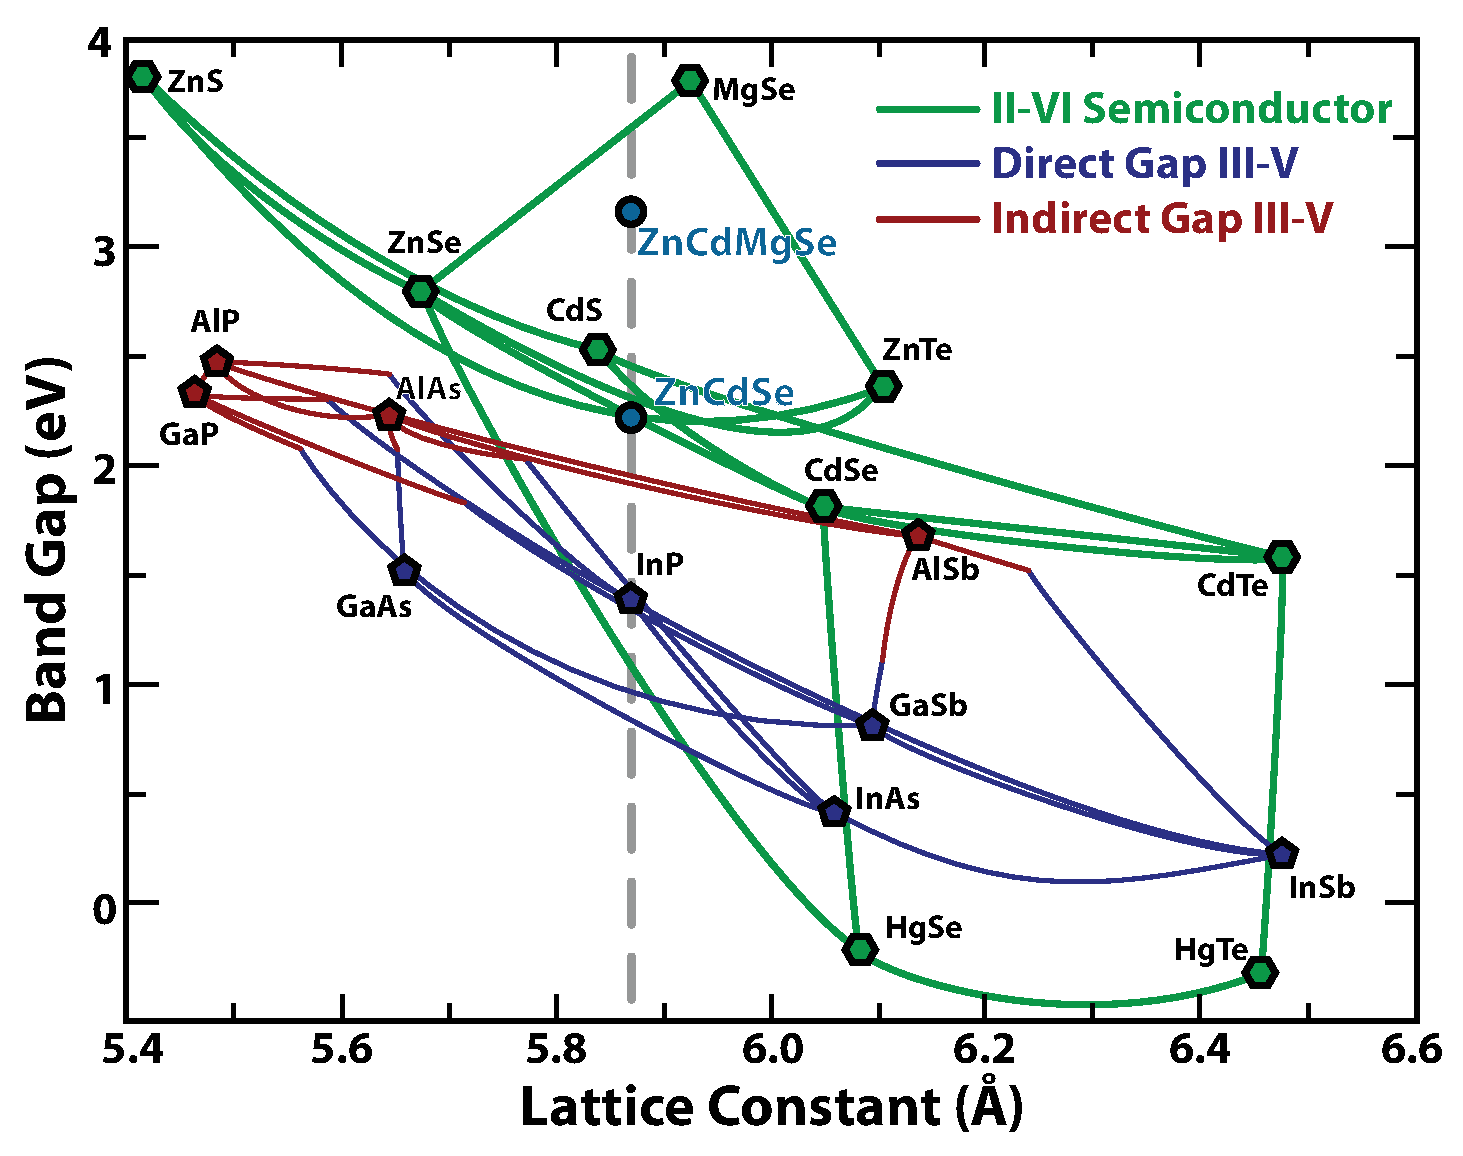
\includegraphics[width=5in]{chpt2/chpt2_gap_v_lattice_iivi}
\caption[Energy gap vs.\ lattice constant for III--V and II--VI materials.]{\textnormal{\textbf{Energy gap vs.\ lattice constant for III--V and II--VI materials.}}  The shortest wavelength QC lasers have been made in III--V systems lattice-matched to InP and InAs.  In this work, we investigate QC sources made from ZnCdSe and ZnCdMgSe.}
\label{chpt2:gap_v_lattice}
\end{figure}

Taking this tactic to the extreme, the field has employed AlAs barrier regions with strategic positioning \cite{Wilison:ElecLett:2001} \cite{Yang:JCQ:2005} \cite{Friedrch:SST:2007} \cite{Revin:APL:2008}
and creative strain compensation strategies \cite{Semtsiv:APL:2004}.
It is at this point we encounter a less obvious constraint to high energy photon generation.  When artificially elevating electrons high up in a semiconductor energy band, as we do with short wavelength QC structures, the full band structure of the semiconductor well and barrier material becomes relevant.  In particular, satellite valleys exist in the $k$-space dispersion of the band structure into which electrons can scatter; such intervalley scattering has been shown to be extremely rapid \cite{Teissier:PRB:1996} \cite{Semtsiv:APL:2008:intervalley}. %Claire comment: add on the order of ... ps, compare to LO phonon scattering and tunneling
When electrons scatter to \emph{k}-space positions away from the $\Gamma$ point, they are effectively trapped in a position that prevents them from participating in population inversion at the $\Gamma$ point.  For example, in QC structures employing lattice-matched In$_{0.53}$Ga$_{0.47}$As as the well material, the energy difference in the conduction band $X$ and $\Gamma$ local minima $\EE_C^X-\EE_C^\Gamma=520$~meV.  Since $\Delta\EE_C=520$~meV for the In$_{0.53}$Ga$_{0.47}$As~/~Al$_{0.48}$In$_{0.52}$As system, using AlAs blocking layers achieves only small gains in photon energy, and here only with strategic positioning of those blocking layers.

Since different materials in our arsenal have different properties, we can attack the satellite valley problem by optimizing the alloy composition we use.  It turns out that between GaAs, AlAs, InAs, and all the ternary compositions between, InAs has the largest $\Gamma$-to-satellite valley offset: $\EE_C^L-\EE_C^\Gamma=0.716$~eV for InAs \cite{Vurgaftman}.  So it comes as no surprise that work in the InAs/AlSb materials system has yielded the shortest wavelength QC lasers to date.  At heat sink temperature $T_{sink}=79$~K, J.~Devenson \emph{et al.} recorded 2.75~\um\ emission ($\EE_{ph}=0.451$~eV) \cite{Devenson:APL:2007}.  This result certainly confirms the restriction that satellite-valley scattering places on the QC emission energy.  QC laser designers typically consider about half of the conduction band offset $\Delta\EE_C$ to be usable for the photon transition, with the remaining offset used for extraneous QC functionality.  The $\Gamma$ point conduction band offset for InAs/AlSb $\Delta\EE_C^\Gamma=2.1$~eV.  With the current, hard-fought emission record at $\EE_{ph}=0.451$~eV, the $\EE_C^L-\EE_C^\Gamma=0.716$~eV restriction is evident.

The community is investigating other materials systems having large conduction band offsets for short wavelength photon generation.  The enormous band gap discontinuities of III--nitrides have not been overlooked \cite{Gmachl:APL:2000:AlGaN}, and attempts have been made to use these for intersubband devices.  %\comment{Switches at telecom wavelengths have been demonstrated [citation].}
GaN-based QC lasers remain elusive, however, primarily due to defects in material quality that lead to problems with vertical transport and current leakage.  Still, work is progressing.  GaN/AlGaN QC structures have shown intersubband photoluminescence at $\lambda$~=~2.13~\um\ \cite{Nevou:APL:2007:AlGaN_EL}, and GaN/AlGaN QC photodetectors have been demonstrated with responsitivity near $\lambda~\approx$~1.7~\um\ \cite{Vardi:APL:2008:AlGaN_detector}. Also, electroluminescence from CdF\sub{2}/CaF\sub{2} QC structures grown on Si has also been reported \cite{Jinen:JJAP:2006}.

%Quantum cascade (QC) development has enabled robust generation of mid-infrared light. To date, the workhorse material for mid-infrared QC lasers has been the InGaAs/AlInAs material system1; lasers from this material have reached the technological benchmark of room temperature, continuous wave operation.2 However, performance is not as advanced at wavelengths below 4 �m. Such high energy photon generation in QC structures is fundamentally limited by the band offset between the well and barrier materials in the relevant carrier transport band. In addressing this fundamental limit, Sb-based III-V heterostructures have demonstrated the shortest wavelength operation to-date achieved for any QC laser: 2.75 �m.3 Sb-based materials are appealing for short-wavelength QC lasers because of their large   valley conduction band-offsets-in InAs/AlSb up to 2.1 eV.4 In this material system, however, scattering out of the upper laser energy state into satellite valleys limits the "effective" usable band offset to ~0.75 eV.4

%Materials systems other than III-V antimonides have been proposed to address the challenges of shorter-wavelength photon generation through intersubband transitions. GaN/AlGaN QC structures have shown intersubband photoluminescence at   ? 2.13 �m,5 and GaN/AlGaN QC photodetectors have been demonstrated with responsitivity near  ? 1.7 �m.6 Electroluminescence from CdF2/CaF2 QC structures grown on Si has also been reported.7

\section{The ZnCdSe/ZnMgSe Materials System}

Evident in Fig.~\ref{chpt2:gap_v_lattice}, II--VI semiconductors open up a whole new world of possibilities for QC structures.  While new to QC lasers, II--VI materials have a substantial history as diode lasers.  Through the 1990s and until the successful demonstration of the InGaN blue laser \cite{Nakamura:JJAP:1996}, II--VI materials looked especially promising as a blue laser and LED source \cite{Tamargo:Book:2002} for consumer products.  For these sources, special attention was paid to the ZnCdSe/ZnMgSe system, due to the especially large band gap of MgSe and the ability to grow ZnMgSe lattice-matched to InP \cite{Tamargo:JEM:1996}.  Interest in the material for laser diodes has seen a resurgence, due to its potential \cite{Guo:APL:1997} to fill the ``green gap'' where InGaN devices with high In concentration are unable to achieve similar levels of performance \cite{DARPA:VIGIL} as their blue-emitting counterparts. Just as III--V QC laser development was able to capitalize on the substantial infrastructure surrounding telecom laser diodes, QC development in II--VI materials is not without infrastructural backing.

\begin{figure}[tp]%
\centering%
%\vspace{0.26in}%
\subfloat[]{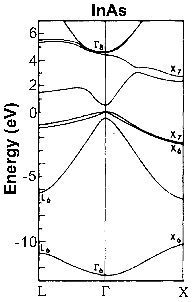
\includegraphics[width=1.9in]{chpt2/chpt2_InAs}%
\label{chpt2:InAs_bd}}%
\hfil%
\subfloat[]{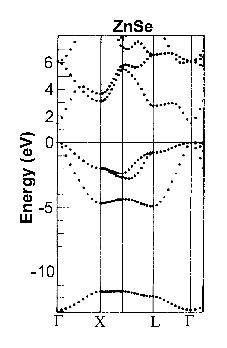
\includegraphics[width=1.9in]{chpt2/chpt2_ZnSe}%
\label{chpt2:ZnSe_bd}}%
\hfil%
\subfloat[]{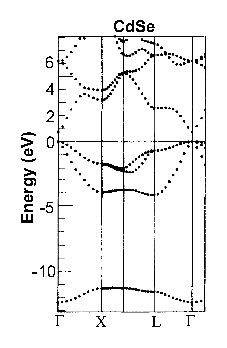
\includegraphics[width=1.9in]{chpt2/chpt2_CdSe}%
\label{chpt2:CdSe_bd}}%
\caption[Bulk energy band diagrams for InAs, ZnSe, and CdSe]{\tn{\textbf{Bulk energy band diagrams for InAs, ZnSe, and CdSe.}}  Band diagrams as calculated by the psuedopotentential method for \tn{(a)} InAs \cite{Chelikowsky:PRB:1976:bulkInAs}, \tn{(b)} ZnSe, and \tn{(c)} CdSe \cite{Zakharov:PRB:1994:bulkZnSe}. The $\EE_C^L-\EE_C^\Gamma$ offsets for InAs, ZnSe, and CdSe are, respectively, $0.716$ \cite{Vurgaftman}, $1.29$, and $1.88~\tn{eV}$ \cite{Zakharov:PRB:1994:bulkZnSe}.  The $\EE_C^X-\EE_C^\Gamma$ offsets for InAs, ZnSe, and CdSe are, respectively, $1.016$ \cite{Vurgaftman}, $1.64$, and $2.27~\tn{eV}$ \cite{Zakharov:PRB:1994:bulkZnSe}.  For GaAs, these values are $0.296$ and $0.462~\tn{eV}$ \cite{Vurgaftman}.  Reprinted with permission from the American Physical Society.}
\label{chpt2:bulk_bds}
\end{figure}

Just as in the blue--green laser diode case, the ZnCdSe/ZnMgSe materials system is appealing for QC structures because of its large band gaps, and---specifically for QC structures---large conduction band offset.  With this material system, we enjoy the added benefit that it can be grown lattice-matched on conventional InP substrate with a zinc-blende crystal structure; for Zn$_{0.43}$Cd$_{0.57}$Se/Zn$_{0.09}$Mg$_{0.91}$Se---the compositions lattice-matched to InP---$\Delta\EE_C^\Gamma$~=~1.2~eV \cite{Sohel:APL:2004}.  In contrast to the large band offset III--V systems, all of the ZnCdSe/ZnMgSe band offset is usable energy space for a QC design.  Figure~\ref{chpt2:bulk_bds} compares calculations of full band structures for ZnSe and CdSe (the component materials of the QC wells) with InAs.  Here, it is evident that the satellite valleys are much higher in the II--VI material.  Indeed, $\EE_C^X-\EE_C^\Gamma~\approx1.64$~eV %2.1~eV for ZnSe %\cite{iivi:25} \cite{iivi:26}
and $\EE_C^\Gamma-\EE_C^X~\approx$~2.27~eV for CdSe \cite{Zakharov:PRB:1994:bulkZnSe}, greater than $\Delta\EE_C^\Gamma$ for the ZnCdSe/ZnMgSe system.

When designing QC structures, the values of several materials properties are needed to fully calculate parameters relevant to a QC design.  In the next sections, I review these values for ZnSe, CdSe, and MgSe, the three relevant component binary materials in the present system.\footnote{One should note that the uncertainty in these parameters is much greater than for III--V systems.}  Ternary compounds---such as Zn\sub{x}Cd\sub{1-x}Se---are often linearly interpolated based on the relative compositions $x$ and $1-x$ of each of the two component binaries ZnSe and CdSe.  More generally, a bowing parameter $C_B$ is sometimes needed to accurately characterize the material property.  For any ternary compound A\sub{x}B\sub{1-x}C, a general material property $G_{ABC}$ is given by
\begin{equation}
G_{ABC}(x) = x \: G_{AC} + (1-x) \: G_{BC} + x \: (1-x) \: C_B \text{.}
\end{equation}
A quaternary material parameter can be calculated by a extending this approach.  For an alloy of type A\sub{x}B\sub{y}C\sub{1-x-y}D, a general property $G_{ABCD}$ is given by
\begin{equation}
G_{ABCD}(x,y) = \frac{y\:(1-x-y)\:G_{ABC}(u) + x\:(1-x-y)\:G_{BCD}(v) + x y \: G_{ACD}(w)}{x y+y\:(1-x-y)+x\:(1-x-y)}
\end{equation}
where $u\equiv 1-\frac{1}{2} x-y$, and $v\equiv 1-x-\frac{1}{2} y$, and $w\equiv(1-x-y)/2$ \cite{Vurgaftman}.

%Alternately, because of magnesium's susceptibility to oxidation, the Zn0.43Cd0.57Se/Zn0.20Cd0.19Mg0.61Se variant is currently more technologically practicable.9 Here, we demonstrate initial steps toward a II-VI QC laser, with the development of a ZnCdSe/ZnCdMgSe QC structure that exhibits intersubband electroluminescence.

%Also include CCNY's previous work on ISB in quantum wells.

%\subsubsection{ZnSe Materials Parameters}
%
%\subsubsection{CdSe Materials Parameters}
%
%\subsubsection{MgSe Materials Parameters}


%\begin{table}[tb]
%\centering
%\doublespacing
%\begin{tabular}{c | c | c | c}
%\hline\hline
%  & ZnSe & CdSe & MgSe \\ \hline
%$a_{\ell c}$ (\AA)  & & & \\
%$C_{11}$ (GPa)  & 88.8\footnotemark[2] & & \\
%$C_{12}$ (GPa)  & 52.7\footnotemark[2] & & \\
%$E_{G}^\Gamma$ (eV)  & 2.82\footnotemark[2] & & \\
%$VBO$ (eV)  & & & \\
%$\Delta_{SO}$ (eV)  & 0.43\footnotemark[2] & 0.42 & 0.40 \\
%$a_c^\Gamma$ (eV)  -5.9\footnotemark[1]& & & \\
%$a_v$ (eV) & -1.0\footnotemark[2] & & \\
%$b$    & -1.14\footnotemark[2]  & & \\
%$m_e^\Gamma$  & 0.15 0.145\footnotemark[2] & 0.11 & 0.23 \\
%%$\gamma_1$  & 2.45 \footnotemark[2] & 1.66 \footnotemark[1] &  \\
%%$\gamma_2$  &  & 0.41 \footnotemark[1] &  \\
%%$\gamma_3$  &  & 0.41 \footnotemark[1] &  \\
%%$E_p$ (eV)  & & & \\
%%$F$  & & & \\
%$\alpha^\Gamma$ (meV/K)  & & & \\
%$\beta^\Gamma$ (K)  & & & \\
%$\epsilon_{s}$ & 8.77\footnotemark[2] 8.8\& 9.2 \footnotemark[1] & \\
%$\epsilon_\infty$ & & 6.0 \footnotemark[1] & \\
%$\hslash \omega_{LO}$ & & & \\
%\hline
%\end{tabular}
%\caption{Materials parameters for ZnSe, CdSe, and MgSe}
%\label{chpt2:table_materials_params}
%\footnotetext[1]{PRB 55, 5184 (1997)}
%\footnotetext[2]{phys. stat. sol. (a) 152, 123 (1995)}
%\footnotetext[3]{PRB 57, 14749 (1998)}
%\end{table}

\begin{table}[tp]
\centering
\begin{minipage}[c]{4in}
\captionsetup{width=4in}
\centering
\setstretch{1.2}
\caption[Material parameters: ZnSe, CdSe, and MgSe]{Materials parameters for ZnSe, CdSe, and MgSe. Source is \cite{Adachi:book:2005}, unless otherwise indicated.  The effective mass is given for the bulk band edge, with $m_0$ the free electron mass.}
\vspace{-0.1in}
\begin{tabular*}{4in}{@{\extracolsep{\fill}} c c c c }%{@{\extracolsep{\fill}} c c p{0.5in} c c }
\toprule
  & ZnSe & CdSe & MgSe\\
\hline
$a_{\ell c}$ (\AA)  & 5.6692 & 6.077 &  5.91\\
$c_{11}$ (GPa)  & 85.7 & 66.7 & 75.8\\
$c_{12}$ (GPa)  & 50.7 & 46.3 & 48.6\\
$\EE_{G}^\Gamma$ (eV)  & 2.721 & 2.07 & 4.0\\
$VBO$ (eV)& 0.53\sup{(1)} & 0.60\sup{(1)} & -0.5\sup{(1)}\\ %  \citesec{Wei:APL:1998}
$\Delta_{SO}$ (eV)  & 0.424  & 0.395  & 0.4  \\
$a_c^\Gamma$ (eV)  & -4.17 & -11.0 &  --- \\
$a_v$ (eV) &  1.65 & -8.9 & -1.0 \\
$b$ (eV)    &  -1.8 & -0.8 & -1.27 \\
$m_e^\Gamma/m_0$  & 0.137 & 0.119 & 0.20 \\
$\alpha^\Gamma$ (meV/K)  & 5.58 & 6.96 & ---\\
$\beta^\Gamma$ (K)  & 187 & 281 & ---\\
$\epsilon_{s}$ & 8.9 & 9.6 & 7.8\\
$\epsilon_\infty$ & 5.9 & 6.2  & 3.8 \\
$\hslash \omega_{LO}$ & 31.2 & 26.2 & 42.2\\% \citesec{iivi:11}
\hline
\end{tabular*}
\singlespacing
\raggedright
\vspace*{-0.18in}
\footnotesize{(1) S.-H. Wei and A. Zunger, \emph{Appl. Phys. Lett.} \tb{72}, 2011 (1998).}
%\label{chpt2:materials_table}
%\bibliographystylesec{kale1}
%\bibliographysec{biblio_iivi}
\end{minipage}
\end{table}

%Claire comment: add in variable names column



\section{Epitaxial Growth of ZnCdSe/ZnMgSe Materials}

The growth of II--VI semiconductors---including ZnCdSe and ZnMgSe---uses the same technological foundation as III--V epitaxial growth.  While most II--VI growth is primarily done with molecular beam epitaxy (MBE) \cite{Tamargo:Book:2002}, metal--organic vapor phase epitaxy (MOVPE) has also been used \cite{Kastner:JCG:1996:iiviMOVPE}.  The three primary binary III--V substrates---GaAs \cite{Haase:APL:1991:ZnSeOnGaAs}, InP \cite{Dai:APL:1995:iiviInP}, and InAs \cite{Litz:JCG:1996:iiviInAs}---have all been used as substrates for II--VI growth, with various II--VI materials that share similar lattice constants.  Both ZnCdSe and ZnMgSe have compositions that match the lattice constant of InP, and with their relatively large conduction band offset of 1.2~eV, the system is highly suitable of QC structures.

The first growth of ZnCdSe on an InP \cite{Dai:APL:1995:iiviInP} substrate had a quite high ($>10^{10}$~cm\sup{-2}) density of stacking faults.  One of the most crucial steps in attaining high quality (low defect density) growth of II--VI materials on III--V substrates is achieving a high quality II--VI/III--V interface.  II--VI growth on InP is particularly challenging.  The standard cleaning method for substrate preparation---an etch such as H\sub{2}SO\sub{4}:H\sub{2}O\sub{2}:H\sub{2}O (7:1:1)---leaves a protective oxide on the substrate surface.  In III--V MBE, the protective oxide is removed in the growth chamber by heating the substrate beyond the oxide desorption temperature.  For InP surfaces, however, because the congruent evaporation temperature of InP (360 $^\circ$C) is less than the oxide desorption temperature (500 $^\circ$C), an As or P overpressure is used to prevent In droplet formation during the oxide desorption process \cite{Cheng:ProcIEEE:1997}.  Here, now, is the problem for II--VI MBE on InP, because As and P sources are not used in a II--VI MBE chamber.  To circumvent this problem, two MBE chambers are used---connected by an ultra-high vacuum (UHV) wafer transfer system.  In the first chamber, a III--V MBE chamber, the oxide desorption procedure under As overpressure is done, and then a high quality \InGaAs buffer layer is grown.  The wafer is transferred under UHV to the second, II--VI MBE chamber, where the II--VI epitaxial growth is then able to proceed.  With the growth of an \InGaAs buffer layer, in addition to a low temperature (170~$^\circ$C) ZnCdSe interfacial layer prior to the main II--VI growth at 270~$^\circ$C, the defect density was reduced to the $10^6$--$10^7$~cm\sup{-2} range \cite{Zeng:APL:1998}.

Once a clean InGaAs surface is achieved, a second problem for growing Se-containing II--VI compounds is encountered.  At the II--VI/III--V heterointerface, the formation of III--VI compounds (Ga\sub{2}Se\sub{3}, for example) are energetically preferred, which themselves form 3D islands rather than a desired 2D growth profile \cite{Li:JVSTB:1994}.  These 3D islands later result in stacking faults that reduce epitaxial quality.  To minimize this interaction, a group II flux (a Zn flux \cite{Zeng:JVSTB:1999:iivi_growth} in the case of ZnCdSe growth) can be used as a III--V surface treatment prior to II--VI growth.  With this additional Zn irradiation step, etch pit defect densities were reduced to the mid $10^4$~cm\sup{-2} range \cite{Zeng:JVSTB:1999:iivi_growth}.

For QC barrier layers, while the growth of lattice-matched ZnMgSe \cite{Sohel:APL:2004} or even strained MgSe \cite{Li:APL:2008:MgSe} is possible, the high Mg content can lead to rapid oxidation and degradation of the epitaxial layers.  For the purposes of initial research into II--VI QC structures, it is more technologically practicable to used quaternary ZnCdMgSe as the QC barrier layers, so as to reduce this oxidation effect.

\section[Intersubband Absorption in ZnCdSe/ZnCdMgSe Quantum Wells]{Intersubband Absorption in ZnCdSe/ZnCdMgSe \\ Quantum Wells}


\begin{figure}[tp]%
\centering%
\subfloat[]{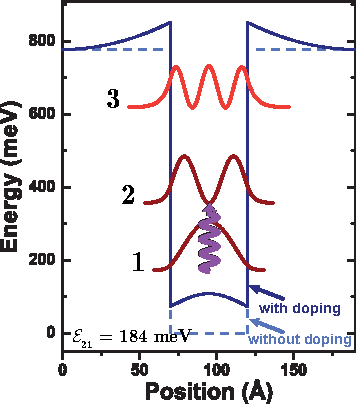
\includegraphics[width=2.12in]{chpt2/chpt2_bdhong}%2.31
\label{chpt2:bdhong}}%
\hfil%
\subfloat[]{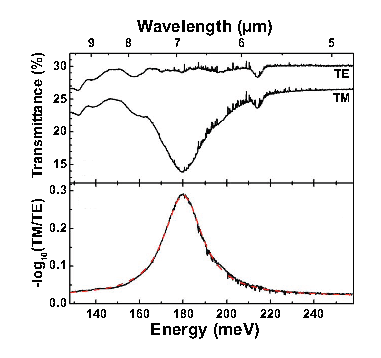
\includegraphics[width=2.9in]{chpt2/chpt2_ISB_transmission}%3.15
\label{chpt2:ISB_transmission_data}}%
\caption[Intersubband absorption of a single quantum structure]{\tn{\textbf{Caption.}} \tn{(a)} Conduction band diagram for a 50.}
\label{chpt2:ISB_transmission}
\end{figure}

As an initial step toward demonstrating ZnCdSe/ZnCdMgSe QC structures, we looked for intersubband absorption in simple single quantum well structures.  The transmission properties at mid-infrared wavelengths of a quantum well sample provide useful information for sample characterization.  If the structure is \emph{n}-type doped, electrons will be available for intersubband absorption out of the ground state in the structure where electrons accumulate.  In a single quantum well structure, this state is just the quantum well ground state.

We looked at intersubband transitions from 50~\AA\ Zn\sub{0.50}Cd\sub{0.50}Se quantum wells surrounded by 140~\AA\ Zn\sub{0.20}Cd\sub{0.19}Mg\sub{0.61}Se barriers \cite{Lu:APL:2006:ISBabs} Cl-doped $n=1\times 10^{18}$~cm\sup{-3}.  The sample was grown with 10 quantum well periods.  The conduction band energy diagram is shown in Fig.~\ref{chpt2:bdhong}, where two quantum well potentials are shown, one that includes the field perturbation from fixed and free charges and one that is only the potential energy of the conduction band edge.  The energy states and wavefunctions (moduli squared) shown include the field perturbation from doping.

%The transitions are then observed as an absorption peak in the transmission spectral data.  For a QC structure with zero applied field, as is usually the case for transmission measurements on QC structures, electrons from the doped injector region typically accumulate in the lowest active region state, since the injector region energy states ``step down'' to the lowest active region state.  This can be seen in Fig.~\ref{chpt2:transmission_bd}, which shows our ZnCdSe/ZnCdMgSe QC structure for $E_\textit{field}=0$~kV/cm.

Transmission data can be taken either in a single-pass configuration, where the wafer is oriented at the Brewster angle relative to the optical axis, or in a multi-pass configuration, where opposing sides of the wafer are polished at a $45^{\circ}$ angle.  In both cases, the wafer back-side (non-epitaxial side) is also mirror-polished.  %The Fig.~\ref{chpt2:transmission_data} inset schematically shows the a wafer in a multi-pass transmission configuration.

Intersubband transitions have transverse magnetic (TM) polarization dependence, since the intersubband energy states result from quantization only in the axis perpendicular to the growth plane.  That is, substantially non-zero optical dipole matrix elements only exist for this $z$ direction.  The polarization dependence of the absorption is useful for transmission data collection.  Since only TM light is absorbed by the quantum wells, transverse electric (TE) light passes through the quantum wells unhindered.  Thus, TE transmission provides an effective ``background'' measurement, where all the properties of detector responsivity, light source spectral intensity, absorption from optical system elements, non-polarization-dependent absorption processes in the semiconductor, etc., are accounted for.  Taking the ratio of the TM and TE spectra, the absorption resulting from intersubband transitions is recovered.

The data in Fig.~\ref{chpt2:ISB_transmission_data}, taken with the sample in a multi-pass configuration, show a single absorption centered near 180~meV.  This is in very good agreement with the model results shown in Fig.~\ref{chpt2:bdhong}, where $\EE_{21}$ is calculated at 184~meV.  The FWHM of the absorption is 20.8~meV, about 11\% of the transition energy, and is an indicator of growth uniformity (InGaAs/AlInAs heterostructures compare at 10\%).



\section{A ZnCdSe/ZnCdMgSe Quantum Cascade Structure}

\begin{figure}[tbp]
\centering
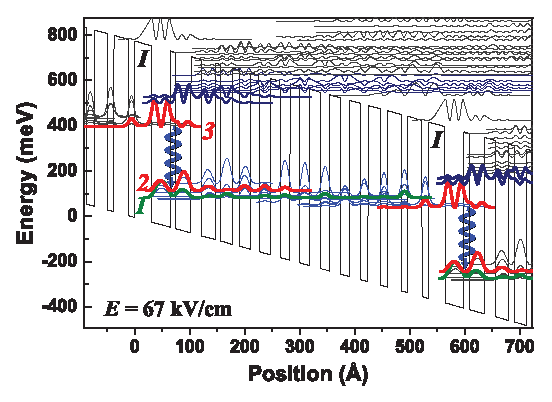
\includegraphics[width=5in]{chpt2/chpt2_band_diagram}
\caption[First generation Zn$_{0.43}$Cd$_{0.57}$Se/Zn$_{0.20}$Cd$_{0.19}$Mg$_{0.61}$Se QC design.]{\tn{\textbf{First generation Zn$_{0.43}$Cd$_{0.57}$Se/Zn$_{0.20}$Cd$_{0.19}$Mg$_{0.61}$Se QC design.}}  A conventional two-well active region QC structure with $L_p=534~\tn{\AA}$. The calculated emission wavelength is $4.37~\tn{\um}$.}
\label{chpt2:band_diagram}
\end{figure}

For a first ZnCdSe/ZnCdMgSe QC structure, our strategy was to design a basic, conventional QC active core.  A design concept that is well-understood in III--V QC structures could then be used as a basis for our data analysis here.  We settled on a simple, two-well active region QC design strategy.  Included in our consideration of design elements was a number of trade-offs.  The larger band offsets afforded by our new material system can support optical transitions with larger photon energies.  But the consequence of larger photon energies is using larger applied electric fields, longer injector regions, or a combination of both.  The relation between these design parameters is quite simply given as
\begin{equation}
E_\textit{field}~=~\frac{\EE_{ph} + \Delta_{inj}}{q L_p} \tn{~.}
\end{equation}
Because it was initially unclear how much field the material system could support, we chose a rather low design turn-on field $E_\textit{field}=67$~kV/cm.  To keep the QC period length $L_p$ reasonably short, we chose a photon energy of 284~meV ($\lambda=4.37$~\um); while relatively large compared to the majority of QC devices, this photon energy is far less than the band offset can in principle  support.

Our conventional two-well active region QC structure was developed with a Zn$_{0.43}$Cd$_{0.57}$Se material composition for the quantum well layers and a Zn$_{0.20}$Cd$_{0.19}$Mg$_{0.61}$Se material composition for the barrier layers. The Fig.~\ref{chpt2:band_diagram} conduction band diagram shows the structure at the design field of 67 kV/cm.  A single stage of the layer sequence is---in angstroms starting from the injection barrier \emph{I}, and going from left to right in the direction of electron flow---\textbf{30} / 34 / \textbf{10} / 28 / \textbf{20} / 24 / \textbf{10} / \underline{22} / \underline{\textbf{12}} / \underline{20} / \underline{\textbf{16}} / \underline{20} / \underline{\textbf{18}} / \underline{18} / \underline{\textbf{18}} / \underline{18} / \underline{\textbf{20}} / \underline{16} / \underline{\textbf{20}} / \underline{16} / \underline{\textbf{20}} / \underline{14} / \textbf{22} / 14 / \textbf{24} / 12 / \textbf{26} / 12. Zn$_{0.20}$Cd$_{0.19}$Mg$_{0.61}$Se barriers are in bold and Zn$_{0.43}$Cd$_{0.57}$Se wells are in normal font. Underlined layers represent ZnCdSe that is Cl-doped $n=2\times 10^{17}$~cm\sup{-3} and ZnCdMgSe doped with the same ZnCl\sub{2} flux as the ZnCdSe layers. We estimate a sheet density per active region--injector period of $n_s=5.4\times 10^{11}$~cm\sup{-2}. The total QC period length $L_p=534$~\AA, and $\Delta_\textit{inj}=74$~meV at $E_\textit{field}=67$~kV/cm.  We calculate an optical dipole matrix element $z_{u\ell}$~=~8.7~\AA.  In the design, an active region energy state is placed 32~meV below the lower optical transition level, sufficient for longitudinal optical (LO) phonon depopulation of the lower laser state via ZnSe- (31.6 meV) \cite{Walsh:PRB:1987} and CdSe-like (26.3 meV) \cite{Yu:SSC:1976} phonons. This configuration results in a calculated upper state lifetime $\tau_u$~=~0.84~ps, lower state lifetime $\tau_\ell$~=~0.21~ps, and non-radiative transition time $\tau_{u\ell}$~=~3.3~ps. Our design calculations included band gaps of 2.08 and 3.03~eV for Zn$_{0.43}$Cd$_{0.57}$Se and Zn$_{0.20}$Cd$_{0.19}$Mg$_{0.61}$Se, respectively, with a conduction band offset of 0.78~eV~\cite{Munoz:APL:2003}. The corresponding conduction band effective masses are calculated to be 0.128 and 0.181 \cite{Munoz:APL:2003} times the free electron mass, respectively.


\section{Device Fabrication \& Processing}

The QC structure was grown by MBE on a low doped
($N<2\times 10^{17}$~cm\sup{-3}) InP:S substrate.  Prior to active core growth, we deposited 0.25~\um\ of \InGaAs (Si-doped $N=5\times 10^{17}$~cm\sup{-3}) as buffer layer. II-VI growth was preceded by a 40~sec Zn flux treatment and 100~\AA\ of low temperature (230 $^{\circ}$C) ZnCdSe (Cl doped $N=2\times10^{17}$~cm\sup{-3}). At the 330 $^{\circ}$C growth temperature, another 400~\AA\ of ZnCdSe (Cl-doped $n=2\times10^{17}$~cm\sup{-3}) buffer was deposited. Ten periods of the active region--injector sequence were grown. The structure was capped by 400~\AA\ ZnCdSe (Cl-doped $n=2\times10^{17}$~cm\sup{-3}) and 2000 \AA\ ZnCdSe (Cl-doped $n=4\times10^{18}$~cm\sup{-3}). Digital transition gradings were used between bulk layers and the active core.

Electroluminescence (EL) structures were fabricated in the form of semicircular cleaved mesas. Two different processes were used, both resulting in devices of similar form.  The first method began with cleaning the epitaxial surface using acetone, isopropanol, and a 1~min, 100~W O\sub{2} plasma at 100~mTorr.  Lithographically-patterned (positive AZ4215E photoresist without image reversal) 400~\um\ diameter circles were etched into mesa structures using a HBr:HNO\sub{3}:H\sub{2}O (1:1:10) wet chemical etch solution; a 1~min, 100~W O\sub{2} plasma descum at 100~mTorr immediately preceded the etch.  The etch depth was sufficient to penetrate the epitaxially grown material (about 3~min of etch time). The sample was again cleaned with acetone, isopropanol, and a 1~min, 100~W O\sub{2} plasma at 100~mTorr.  A second lithography step (negative AZ4215E photoresist with image reversal) was used to define a lift-off pattern for the top contact metallization, which consisted of 350~\um\ diameter circles centered on the etched 400~\um\ diameter mesas.  The wafer surface was cleaned and prepared for metalization with a 30~sec, 100~W O\sub{2} plasma descum at 100~mTorr followed by a 45~sec HF:H\sub{2}O (1:1) dip to remove surface oxide.  These cleaning steps immediately preceded top metal contact deposition.  Top contacts consisted of 150~\AA\ Ti followed by 2500~\AA\ Au \cite{Miyajima:JJAP:1992:TiAu_contacts}; Ge/Au back-side InP contacts were also deposited.

A second mesa processing method yielded far more consistent results, especially with regard to repeatable, high quality, ohmic, and mechanically stable top (epitaxial-side) metal contacts.  The first processing step was applying the top metal contact, and then the remaining mesa processing steps followed.  Processing began with an epitaxial surface cleaning, consisting of acetone, isopropanol, and a 1~min, 100~W O\sub{2} plasma at 100~mTorr.  Surface oxides were removed with a 5~min HCl:H\sub{2}O (1:1) etch\footnote{It is worth noting that concentrated HCl etches the II--VI epitaxial layers.  HCl that is diluted with equal part H\sub{2}O, however, has no appreciable etching of the II--VI epitaxial layer after 5~min, and is thought to be effective at removing surface oxides. %Claire comment: needs a reference
} \cite{Miyajima:JJAP:1992:TiAu_contacts}, which immediately preceded application of the epitaxial-side metals.  The top contact metal layers were 150~\AA\ Ti followed by 2500~\AA and were e-beam evaporated across the entire surface.  A first lithography step (positive AZ4215E photoresist without image reversal) consisted of 350~\um\ diameter circles and was used to define the boundaries of the top metal contacts.  An iodine-based Au etch at 25~$^{\circ}$C sufficiently removed the unwanted Au after 3~min; the Ti adhesion layer not removed by the Au etch was removed after 15~sec in concentrated HF, effective due to the rapid oxidation of Ti.  The sample was again cleaned with acetone, isopropanol, and a 1~min, 100~W O\sub{2} plasma at 100~mTorr.  A second lithography step (positive AZ4215E photoresist without image reversal) consisting of 400~\um\ diameter circles centered over the 350~\um\ diameter Au circles was used to define the boundaries for the mesa etch.  A 1~min, 100~W O\sub{2} plasma descum at 100~mTorr was used to prepare for the mesa etch.  Mesas were etched using a HBr:HNO\sub{3}:H\sub{2}O (1:1:10) solution; the etch depth was sufficient to penetrate the epitaxially grown material (about 3~min of etch time).  Finally, the remaining photoresist was stripped with acetone and isopropanol.  A back-side Ge/Au contact was also supplied similar to the first method.

After both processes, the mesas were cleaved into semicircular EL structures and In soldered to Cu heat sinks.  The top electrical contacts were wire bonded to contact pads. %Cleaved mesa areas were measured as around 0.036 mm2.

\section{Measurements and Data}
\label{chpt2sec:data}

\subsection{Quantum Cascade Intersubband Absorption}

We again characterized our QC structure using a multi-pass transmission measurement, schematically depicted in the Fig.~\ref{chpt2:transmission_data} inset.  For a QC structure with zero applied field, as is usually the case for transmission measurements on QC structures, electrons from the doped injector region typically accumulate in the lowest active region state, since the injector region energy states ``step down'' to the lowest active region state.  This can be seen in Fig.~\ref{chpt2:transmission_bd}, which shows our ZnCdSe/ZnCdMgSe QC structure for $E_\textit{field}=0$~kV/cm.

\begin{figure}[tp]%
\centering%
\subfloat[]{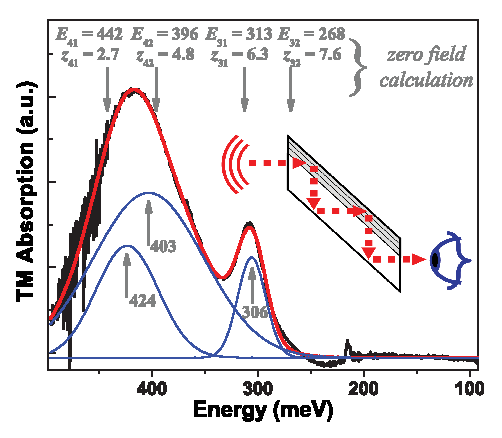
\includegraphics[width=3.2in]{chpt2/chpt2_absorption}%
\label{chpt2:transmission_data}}%
\hfil%
\subfloat[]{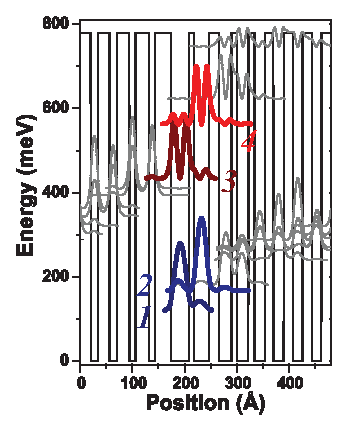
\includegraphics[width=2.21in]{chpt2/chpt2_zerofield_bd}%
\label{chpt2:transmission_bd}}%
\caption[TM absorption spectrum from multi-pass transmission]{\tn{\textbf{TM absorption spectrum from multi-pass transmission.}} \tn{(a)} Fitted Gaussians show three resolvable peaks. Optical transition calculations for zero applied field are indicated at the top. The inset shows the multi-pass configuration with broadband light passing through a sample polished to $45^{\circ}$ on both ends. \tn{(b)} The QC conduction band structure at $E_\tn{\textit{field}}=0~\tn{kV/cm}$.  Electrons from the doped injector relax to and accumulate in the state labeled \tn{\textit{1}}.}
\label{chpt2:transmission_figs}
\end{figure}


%Transmission data can be taken either in a single-pass configuration, where the wafer is oriented at the Brewster angle relative to the optical axis, or in a multi-pass configuration, where opposing sides of the wafer are polished at a $45^{\circ}$ angle.  In both cases, the wafer back-side (non-epitaxial side) is also mirror-polished.  The Fig.~\ref{chpt2:transmission_data} inset schematically shows the a wafer in a multi-pass transmission configuration.

%Intersubband transmissions have TM polarization dependence, since the intersubband energy states result from quantization only in the axis perpendicular to the growth plane.  That is, optical dipoles matrix elements only exist for this $z$ direction.  The absorption polarization dependence is useful for transmission data collection.  Since only TM light is absorbed by the quantum wells, TE light passes through the quantum wells unhindered.  Thus, TE transmission provides an effective ``background'' measurement, where all the properties of detector responsivity, light source spectral intensity, absorption from optical system elements, etc., are accounted for.  Taking the ratio of the TM and TE spectra, the absorption solely resulting from intersubband transitions is recovered.

The absorption spectrum of our structure shows two dominant TM peaks, shown in Fig.~\ref{chpt2:transmission_data}.  For these two peaks, three Gaussian curves---centered at 306, 403, and 424~meV---provide an accurate fit.  We calculate potential optical transitions for the zero field structure at 268, 313, 396, and 442~meV, as indicated in Fig.~\ref{chpt2:transmission_data}.  These calculations are largely consistent with the observed absorption.

\subsection{Electroluminescence Spectra}

\begin{figure}[tbp]
\centering
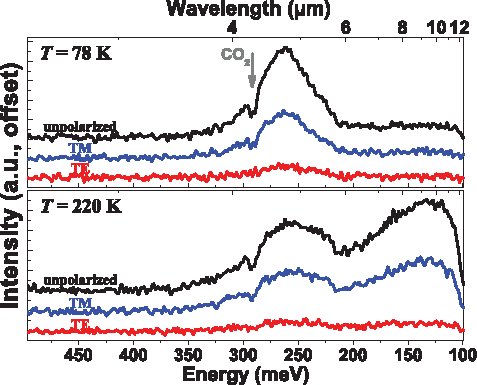
\includegraphics[width=4.25in]{chpt2/chpt2_polarized_emission}
\caption[Polarization-resolved EL spectra]{\tn{\textbf{Polarization-resolved EL spectra.}}  The data is for a device driven with $9.6~\tn{kA/cm}^2$ at $78~\tn{K}$ (top) and $220~\tn{K}$ (bottom). The emission is predominantly TM polarized.  Additional longer wavelength light is seen at higher heat sink temperatures and currents.  Atmospheric CO\sub{2} absorption can be seen near $\lambda=4.2~\tn{\um}$. Spectra are not corrected for detector responsivity, which is more sensitive at longer wavelengths.}
\label{chpt2:spectra_polarization}
\end{figure}

Electroluminescence was collected for a variety of heat sink temperatures and applied current values using a Fourier transform infrared (FTIR) spectrometer in step scan mode and a cooled HgCdTe detector. The applied current pulses were 1~\textmu s in duration at 3\% duty cycle.

\begin{figure}[tbp]
\centering
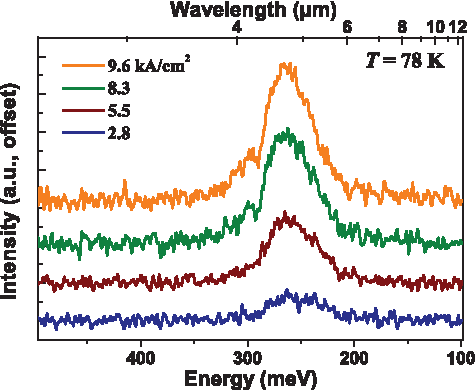
\includegraphics[width=4.25in]{chpt2/chpt2_80K_emission}
\caption[EL spectra at $T=78~\tn{K}$]{\tn{\textbf{EL spectra at \textit{T}=78~K.}} Spectra at various current levels
are shown.  Emission intensity increases with increasing current.  Emission is centered near $4.8~\tn{\um}$.}
\label{chpt2:spectra_78K}
\end{figure}

We observed EL centered near $\lambda=4.8$~\um (258~meV). Emission polarization characteristics were examined to confirm intersubband light generation. Two exemplary results of polarization-resolved EL spectra are shown in Fig.~\ref{chpt2:spectra_polarization} for heat sink temperatures of 78~K and 220~K and a pumping current of 9.6~kA/cm\sup{2}. While a small amount of TE light is observed, which we attribute to scattering from within the rounded mesa, the EL is predominantly TM polarized.

At low temperatures, the primary emission peak is observed near 4.8~\um. Figure~\ref{chpt2:spectra_78K} shows emission behavior with increasing current for a heat sink temperature of 78~K and no polarizer in the optical path. The 4.8~\um\ emission peak grows correspondingly with increasing pumping current. At a pumping current density of 2.8~kA/cm\sup{2}, a Gaussian fit gives an EL full-width at half-maximum (FWHM) of 52~meV; at 9.6~kA/cm\sup{2} the FWHM is 47~meV, which is about 20\% of the transition energy.

\begin{figure}[tbp]
\centering
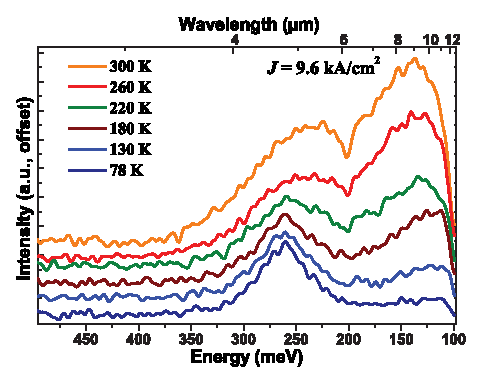
\includegraphics[width=4.25in]{chpt2/chpt2_9p6kacm_emission}
\caption[Temperature-dependence of EL spectra]{\tn{\textbf{Temperature-dependence of EL spectra.}}  EL spectra are at $9.6~\tn{kA/cm}^2$ for heat sink
temperatures from $78$ to $300~\tn{K}$. Additional longer-wavelength light is seen with increasing temperature. Over the $78$ to $300~\tn{K}$ temperature range, the $4.8~\tn{\um}$ peak intensity decreases by $30\tn{\%}$ and emission width increases by $36\tn{\%}$. Spectra are not corrected for variations in detector responsivity, which is more sensitive at longer wavelengths.}
\label{chpt2:spectra_alltemps}
\end{figure}

This 4.8~\um\ light is seen at temperatures ranging from 78 to 300~K. Figure~\ref{chpt2:spectra_alltemps} shows spectra with increasing temperature for a pumping current density of 9.6~kA/cm\sup{2}. All spectra represent TM polarized light with subtraction of the corresponding unpolarized background. The emission peak centered near 4.8~\um\ is present over the full temperature range. We also observed the growth of a secondary, temperature-induced, lower energy emission. This broad emission is more intense for both higher currents and higher temperatures. Reported spectra are not corrected for wavelength-dependent variations in detector responsivity; we estimate our detector is 55\% more sensitive for 120~meV photons than for 260~meV photons. While the origin of this low energy emission remains unclear, the 4.8~\um\ emission is dominant and persists through room temperature. This emission has the well-known temperature-dependent behavior: from 78 to 300~K, Gaussian fits that include a rising background show that peak intensity decreases by 30\% and emission width increases by 36\%.

\subsection{Light--Current--Voltage Data}

\begin{figure}[tbp]
\centering
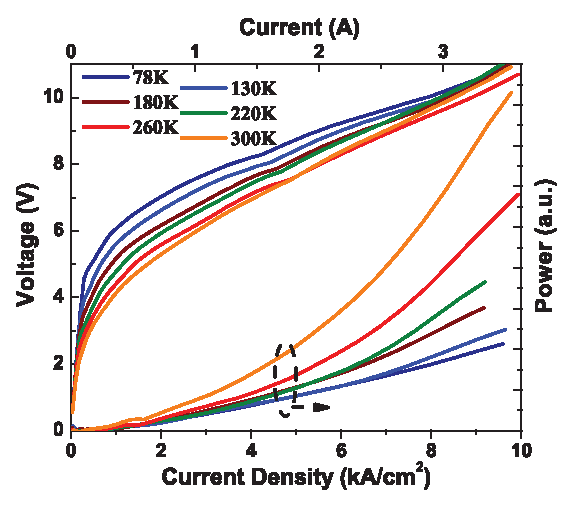
\includegraphics[width=4.25in]{chpt2/chpt2_liv}
\caption[EL structure LIV]{\textbf{EL structure LIV.}  Spectrally integrated light--current--voltage data from $78$ to $300\tn{K}$.
The data were collected with $1~\tn{\textmu s}$ pulses at $3$\% duty cycle. Data are not corrected for detector responsivity.}
\label{chpt2:LIV}
\end{figure}

Figure~\ref{chpt2:LIV} shows wavelength-integrated light--current--voltage (LIV) measurements for temperatures ranging from 78 to 300~K. The light-current (LI) data represent TM polarized emission. The observed output power grows superlinearly for both increasing current and increasing temperatures. The current-voltage (IV) curves show typical QC behavior, with characteristic current turn-on once sufficient voltage has been applied.  Turn-on for 78~K occurs at 5.40~V. At a turn-on field of 64~kV/cm, 3.42~V is dropped over the active core. We attribute to conduction band offsets at bulk interfaces another 0.35~V. The remaining 1.63~V is likely dropped over the as yet non-ideal top contacts.

\section{Second-Generation Design}

\begin{figure}[tbp]
\centering
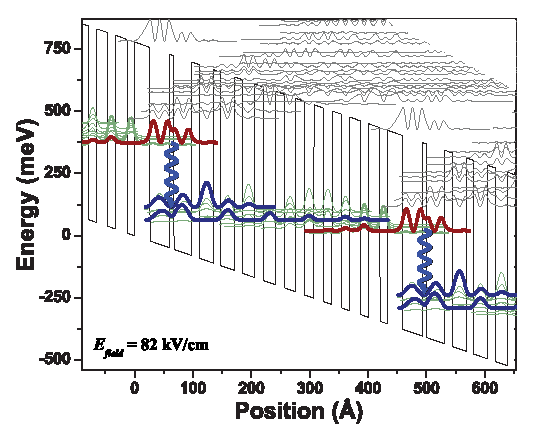
\includegraphics[width=5in]{chpt2/chpt2_new2well_bd}
\caption[Second generation Zn$_{0.43}$Cd$_{0.57}$Se/Zn$_{0.20}$Cd$_{0.19}$Mg$_{0.61}$Se QC design.]{\textbf{Second generation Zn$_{0.43}$Cd$_{0.57}$Se/Zn$_{0.20}$Cd$_{0.19}$Mg$_{0.61}$Se QC design.}  A conventional two-well active region QC structure with $L_p$~=~534~\AA, calculated emission is 4.88~\um.}
\label{chpt2:2nd_bd}
\end{figure}

With our initial demonstration of EL, we sought to improve upon the result with an improved QC structure.  While we indeed observed some EL, the intensity of the emission was extremely weak.  And because of such weak emission, we would not expect to see lasing from the structure, or even the presence of gain.  One fundamental problem with the design was an energy spacing between the lowest active region states that is very nearly equal to the LO phonon energy; if the active region barrier ended up being only marginally too large, the LO phonon scattering channel out of the lower laser state would be slowed down considerably and population inversion would be extremely difficult.  Another fundamental problem was the ``tight'' (in energy range) injector that may have limited the amount of current able to be pushed through the device.

In a second generation design, we sought to mitigate these problems.  We grew more periods: 25, instead of 10.  We also improved the design, which is shown in Fig.~\ref{chpt2:2nd_bd}.  In this design, the period length has been decreased slightly to $L_p=432$~\AA\ and the field increased to $E_{field}=82$~kV/cm.  Also, the energy splitting between the lowest to active region states has been increased to 58~meV, to provide room for error in the active region barrier thickness.  The layer sequence is, in angstroms starting from the injection barrier, \textbf{26} / 34 / \textbf{6} / 30 / \textbf{14} / 24 / \textbf{12} / \underline{24} / \underline{\textbf{14}} / \underline{20} / \underline{\textbf{16}} / \underline{20} / \underline{\textbf{16}} / \underline{18} / \underline{\textbf{16}} / \underline{16} / \underline{\textbf{16}} / \underline{15} / \underline{\textbf{16}} / \underline{14} / \underline{\textbf{18}} / \underline{14} / \textbf{20} / 13.  The as-designed photon energy is $\EE_{u\ell}=254$~meV ($\lambda=4.88$~\um).  Zn$_{0.20}$Cd$_{0.19}$Mg$_{0.61}$Se barriers are in bold and Zn$_{0.43}$Cd$_{0.57}$Se wells are in normal font. Underlined layers represent ZnCdSe that is Cl-doped $n=3\times 10^{17}$~cm\sup{-3} and ZnCdMgSe doped with the same ZnCl\sub{2} flux as the ZnCdSe layers.

After growth and processing as previously described, we examined EL spectral data for the device.  The spectral emission was remarkably similar to that in Fig.~\ref{chpt2:spectra_alltemps}, with the emission peaks looking nearly identical between the first and second generation devices.  The low-energy thermal emission was also both present and similar in the second generation device.  This, even though the design wavelengths between the first and second generation devices were nominally different: 4.37 vs.\ 4.88~\um, respectively.  The origins of the similarities remain under investigation, and the finding certainly adds a degree of doubt that the source of the EL is intersubband in nature.  Notwithstanding this result, much of the original evidence for the first generation device indeed still points to an intersubband transition as the EL source; the polarized emission, the growing peak intensity with pumping current, and the conventional-looking IV curves, for example, all suggest a functioning QC device.

\section{Conclusions \& Future Directions}
\subsection{Summary}

With this work in II--VI heterostructures, we have laid a foundation for a new class of QC lasers.  The successful demonstration of a II--VI QC laser would be an important milestone; as the first QC laser outside of a III--V materials system, a II--VI QC laser would truly demonstrate the overtly unencumbered flexibility of the quantum cascade.  %And while QC Only needing a narrow bandgap material and a wide bandgap material to to form the engineered, ``artificial'' bandgap of an emitter.

In the work presented here, we have shown progress toward demonstrating such II--VI QC lasers.  We have developed the capability to design II--VI QC structures, which is able to both accurately reproduce observed data from simple single quantum well samples as well as facilitate II--VI QC design development.  A typical first step toward the fabrication of intersubband devices is demonstrating intersubband absorption from simple quantum well structures, which we have done.  The processes associated with the fabrication of optoelectronic devices often presents a challenge, and we have developed reliable fabrication methods for our II--VI devices. %;, including a reliable method for making contacts.
With regard to QC design, we have developed and grown several structures.  From these, we have seen intersubband absorption that is in good agreement with calculated absorption energies.  Moreover, we have observed TM-polarized electroluminescence, with emission at a wavelength in good agreement with the design.  While recent data brings into question the source of the EL (whether it is intersubband or of some other origin), the IV curves from these devices are further supporting evidence that we have QC structures with properly functioning electron transport.


\subsection{Future Direction: New II--VI design strategies}

Immediate future work will focus on several new design strategies.  The growth of ZnCdSe / ZnCdMgSe structures presents a considerable materials and engineering challenge.  II--VI QC growth engineers must be even more skilled and accurate in their calibrations than III--V growth engineers.  The larger effective mass of II--VI materials means that equivalent errors in layer thickness between the two systems results in a much more significant variation of the quantum well band structure for the II--VI device; simply put, there is less room for error.

While the demands on the II--VI growth effort are large, QC designers can help the process with designs that are specifically aimed at making the growth engineer's job easier.  Two new design strategies---superlattice QC structures and using less wells in the QC period---may mitigate some of the challenges specifically faced by the II--VI material system.

%However, we can help the growers out with some new and better design innovations.  All about making growth easier
%
%fewer wells (increase field), also a two phonon structure
%
%superlattice
%
%increase photon energy, may improve emission, prove that first demonstration was real

\subsubsection{ZnCdSe/ZnCdMgSe superlattice QC structures}

A superlattice QC structure \cite{Scamarcio:Science:1997:superlattice} is fundamentally different from other QC structures.  In superlattice structures, many more quantum well and barrier layers are used for each QC period, with each layer much narrower by comparison.  Superlattice QC structures create a ``miniband'' of states, in contrast to the more discrete nature of states in conventional QC structures.  One marked advantage of superlattice structures, especially for II--VI QC growth, is that the thickness of any individual layer is not nearly as critical.

\begin{figure}[tbp]
\centering
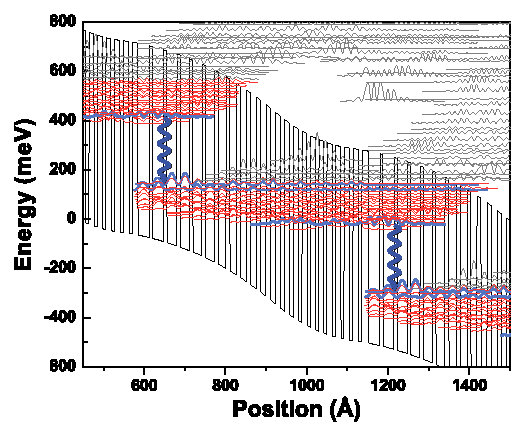
\includegraphics[width=4.25in]{chpt2/chpt2_sl_bd}
\caption[Superlattice ZnCdSe/ZnCdMgSE QC structure]{\tn{\textbf{Superlattice ZnCdSe/ZnCdMgSE QC structure.}}  Superlattice structures have the advantage that the thickness of any individual layer is not as crucial, which may make the structure easier to grow.  This structure, designed in the Zn$_{0.43}$Cd$_{0.57}$Se / Zn$_{0.20}$Cd$_{0.19}$Mg$_{0.61}$Se materials system, has a designed photon energy $\EE_{ph}=275~\tn{meV}$ ($\lambda_0=4.52~\tn{\um}$) at an applied field $E_\tn{\textit{field}}=70~\tn{kV/cm}$.  Band bending of the superlattice structure is seen, resulting from a self-consistent calculation that accounts for energy state positions with the band effects of fixed and free charge.}
\label{chpt2:sl_bd}
\end{figure}

An example of a superlattice QC structure using Zn$_{0.43}$Cd$_{0.57}$Se quantum wells and Zn$_{0.20}$Cd$_{0.19}$Mg$_{0.61}$Se is shown in Fig.~\ref{chpt2:sl_bd} for an applied field of 70~kV/cm. In angstroms starting from the injection barrier, the layer sequence is \textbf{14} / 29 / \textbf{8} / 27 / \textbf{8} / 25 / \textbf{8} / 23 / \textbf{8} / 23 / \textbf{8} / 22 / \textbf{10} / 20 / \textbf{9} / 17 / \textbf{9} / 16 / \textbf{10} / 15 / \textbf{11} / 14 / \textbf{11} / 12 / \textbf{12} / 12 / \textbf{12} / 11 / \textbf{12} / 10 / \textbf{12} / 10 / \textbf{12} / 9 / \textbf{12} / 8 / \textbf{13} / 8 / \textbf{13} / 8 / \textbf{14} / 7 / \textbf{14} / 7, where Zn$_{0.20}$Cd$_{0.19}$Mg$_{0.61}$Se barriers are in bold font and Zn$_{0.43}$Cd$_{0.57}$Se wells are in normal font.  Clearly, this structure contains many more layers than a comparable conventional design, here 44 compared to 28 in Fig.~\ref{chpt2:band_diagram} which has a similar photon energy.  However, the overall period length, 573~\AA\ compared to 534~\AA, is not significantly different, so the thickness of the epitaxial growth is about the same.

\subsubsection{Fewer layers per QC period}

While the superlattice QC structure can make the growth task easier by lessening the importance of individual layer thicknesses, another approach is to decrease the number of layers altogether.  By doing this, we can have the same number of photon transitions for a shorter growth time and smaller growth thickness, or equivalently, have more photon transitions for the same epitaxial growth thickness.

\begin{figure}[tbp]
\centering
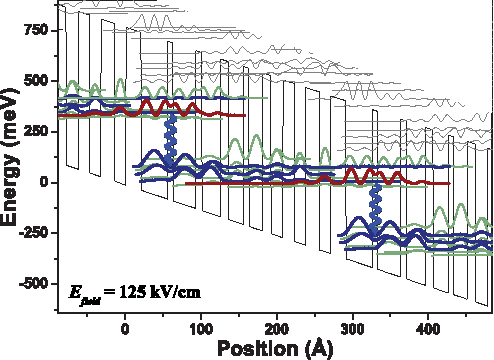
\includegraphics[width=4.25in]{chpt2/chpt2_bd4900}
\caption[ZnCdSe/ZnCdMgSE QC structure with fewer layers]{\tn{\textbf{ZnCdSe/ZnCdMgSE QC structure with fewer layers.}}  Compared to the first generation design shown in Fig.~\ref{chpt2:band_diagram} with 28 well and barrier layers, this design has 16 layers for a similar photon energy of $\EE_\tn{\textit{ph}}=255~\tn{meV}$ ($\lambda_\tn{0}=4.86~\tn{\um}$).  The trade-off is that the field is substantially increased.}
\label{chpt2:bd4900}
\end{figure}

The trade-off here, as explained earlier in this chapter, is that a shorter QC period requires a larger applied electric field for any given optical transition energy.  However, through the earlier results of this work, we are confident that this II--VI material system can indeed withstand larger fields.  As an example, increasing the field to $E_\textit{field}=125$~kV/cm for a $\sim\!250$~meV photon transition (as in Fig.~\ref{chpt2:band_diagram}), shortens the period length from 534~\AA\ to 270~\AA.  Specifically, the structure in Fig.~\ref{chpt2:bd4900} has a layer sequence, in angstroms starting from the injection barrier, \tb{20} / 35 / \tb{7} / 30 / \tb{8} / 25 / \tb{10} / 20 / \tb{7} / 18 / \tb{11} / 16 / \tb{15} / 15 / \tb{18} / 15, where Zn$_{0.20}$Cd$_{0.19}$Mg$_{0.61}$Se barriers are in bold font and Zn$_{0.43}$Cd$_{0.57}$Se wells are in normal font.  With only 16 layers compared to 28 per QC period, growth may be simplified for this structure.

\subsubsection{QC structure with larger photon energy}


\begin{figure}[tbp]
\centering
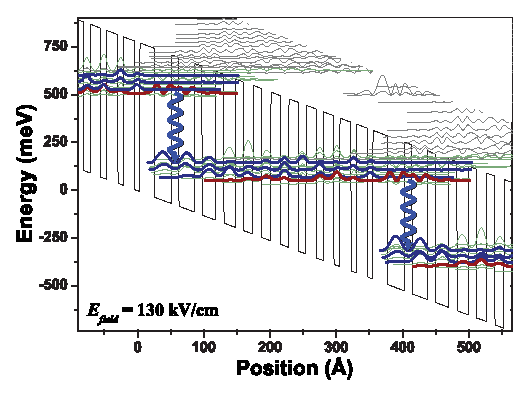
\includegraphics[width=4.25in]{chpt2/chpt2_bd3350}
\caption[Short wavelength ZnCdSe/ZnCdMgSE QC structure]{\tn{\textbf{Short wavelength ZnCdSe/ZnCdMgSE QC structure.}}  Investigating a higher photon energy QC structure may be beneficial.  Here, a $\EE_\tn{\textit{ph}}=370~\tn{meV}$ ($\lambda_\tn{0}=3.35~\tn{\um}$) structure achieved using Zn$_{0.43}$Cd$_{0.57}$Se quantum wells and Zn$_{0.20}$Cd$_{0.19}$Mg$_{0.61}$Se barriers.}
\label{chpt2:bd3350}
\end{figure}

An open question in the work presented is the true origin of the observed EL described in Section~\ref{chpt2sec:data}.  Due to the similar (but not the same) wavelengths of the first (Fig.~\ref{chpt2:band_diagram}) and second (Fig.~\ref{chpt2:2nd_bd}) generation designs, the similarity in emission may be simply result from the emission being broad.  To test this theory and confirm that we have truly demonstrated intersubband QC EL, a structure that substantially changes the photon energy will be helpful.  In a larger photon energy structure, the emission may be easier to observe due to the larger output powers resulting from more energy per photon.

While today's QC designs seek to have ample confinement of the upper laser state within the quantum wells to prevent thermal escape,  there have been numerous examples where this is not the case \cite{Faist:APL:1998:short}, \cite{Faist:APL:1995:Bragg}.  And indeed, if one is looking for only low temperature emission, having the upper laser state deeply confined in the quantum wells is not necessary.  As an example, Fig.~\ref{chpt2:bd3350} shows a design for a $\lambda_0=3.35$~\um\ QC structure.  The layer sequence, in angstroms from the injection barrier, is \tb{22} / 26 / \tb{11} / 23 / \tb{12} / 20 / \tb{13} / 17 / \tb{12} / 15 / \tb{13} / 14 / \tb{14} / 13 / \tb{15} / 11 / \tb{16} / 10 / \tb{16} / 9 / \tb{17} / 8 / \tb{17} / 8, with Zn$_{0.20}$Cd$_{0.19}$Mg$_{0.61}$Se barriers in bold font and Zn$_{0.43}$Cd$_{0.57}$Se wells in normal font.  Here, even with a substantially larger photon energy ($\EE_{ph}=370$~meV), the QC period length is still kept to a relatively low 352~\AA.

\subsection{Future Direction: Strain-compensated growth}

While increasing the Mg content from the current $x=61$\% mole fraction (Zn$_{0.20}$Cd$_{0.19}$Mg$_{0.61}$Se) to the lattice-matched 91\% mole fraction (that is, using Zn\sub{0.09}Mg\sub{0.91}Se) in the barrier layers would support substantially larger photon energies for shorter wavelength generation, another approach might be to incorporate strain.  Much as strain compensation has been used for InGaAs / AlInAs structures in III--V QC lasers, we could use a similar concept for ZnCdSe / ZnCdMgSe.  The InGaAs and AlInAs materials are well-suited to this scheme, since both have bandgaps that increase with compositions that lead to tensile strain and decrease with compositions that lead to compressive strain.  When looking at only ZnCdSe and ZnMgSe materials (not including the quaternary ZnCdMgSe), using strain compensation does not appear possible; like InGaAs and AlInAs, ZnCdSe has a bandgap that decreases with compositions that lead to compressive strain, but ZnMgSe is just the opposite.  Therefore, adding tensile strain to one material and compressive strain to the other material in the ZnCdSe/ZnMgSe system will always lead to smaller band offsets.  However, with the quaternary ZnCdMgSe, we gain an extra degree of freedom in material composition that again allows strain compensation to be beneficial to increasing the band offset.  Thus, strain compensation could be used in the current ternary/quaternary II--VI system without the inclusion of substantially more Mg that in turn leads to growth and reliability challenges from Mg oxidation.

\subsection{Future Direction: Fabrication of II--VI QC laser waveguides}

When it comes to fabricating laser ridges from our II--VI materials grown on InP, we confront a challenge.  With a refractive index in the II--VI materials that is substantially lower than that of the III--V materials, creating a waveguide that supports an optical mode with a high gain region confinement factor cannot be done using the traditional methods. In conventional QC lasers grown in InP, the active core has a larger refractive index than the InP cladding, so the mode is easily confined in the active core.  Conversely, with II--VI on InP, we have a situation similar to that confronted by InAs/AlSb QC lasers and GaAs/AlGaAs lasers.  These devices overcome the challenge by growing thick buffer or superlattice cladding confinement layers, or using in-cladding doping to reduce the refractive index (plasmon-enhanced waveguides).

\begin{figure}[tbp]
\centering
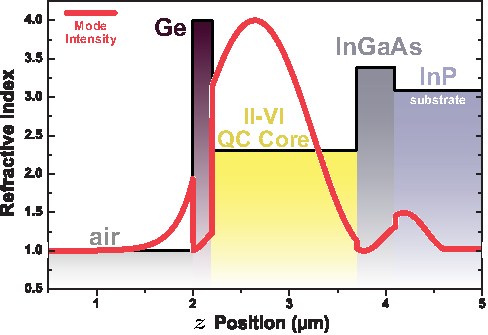
\includegraphics[width=4.25in]{chpt2/ge_wg}
\caption[II--VI QC waveguide]{II--VI QC waveguide.  Because of the low refractive index of II--VI materials relative to InP, making high confinement waveguides for the active II--VI region is difficult.  One possible solution is using a Ge top cladding that is deposited during laser ridge fabrication.  As shown here for 4.2~\um\ light, this structure is capable of guiding an optical mode.}
\label{chpt2:ge_wg}
\end{figure}

Growing optically thick buffer layers of II--VI materials may prove difficult. However, waveguides can still be made.  One solution is using a high index \InGaAs buffer grown on InP to hold the optical mode; here the II--VI active gain layers would just be off the mode center, and we will have to accept a lower confinement factor.  Yet, we may be able to do better.  QC lasers using air as waveguide top cladding have been demonstrated by Moreau \emph{et al.} \cite{Moreau:OptExp:2007:air_guide}, ostensibly in their work for evanescent wave sensing using the optical mode of the laser cavity.  Also, as suggested (for example) by  Almeida \emph{et al.} \cite{Almeida:OL:2004}, modes can be supported in a low index material that is sandwiched between two high index materials, given proper geometries and dimensions for the supported wavelength.  For a II--VI QC laser, we can create a high confinement waveguide that symmetrically encompasses the QC active core by using \InGaAs as a high index bottom cladding and evaporated Ge as a high index top cladding after initially fabricating the laser ridge with an air top cladding.  The mode profile for such a structure is shown in Fig.~\ref{chpt2:ge_wg}.



%
%\bibliographystyle{kale3}
%%\bibliography{../short_inj/KaleAbrv,biblio}
%\bibliography{biblio}
%
%
%
%\end{document} 